\documentclass[aspectratio=169]{beamer}
% Add slides directory to search path for Dartmouth theme
\makeatletter
\def\input@path{{../}}
\makeatother
\usetheme{Dartmouth}
\usepackage{booktabs}
\usepackage{listings}
\usepackage{tikz}
\usepackage{hyperref}
\usepackage{xcolor}
\usepackage{graphicx}
\usepackage{fontspec}
% Color scheme
\definecolor{darkblue}{RGB}{0,82,155}
\definecolor{lightblue}{RGB}{100,181,246}
\definecolor{darkgreen}{RGB}{46,125,50}
\definecolor{orange}{RGB}{255,152,0}

\setbeamercolor{frametitle}{bg=darkblue}
\setbeamercolor{progress bar}{fg=lightblue,bg=lightblue!30}

% Code listing settings
\lstset{
    basicstyle=\ttfamily\small,
    breaklines=true,
    frame=single,
    backgroundcolor=\color{gray!10},
    keywordstyle=\color{darkblue}\bfseries,
    commentstyle=\color{darkgreen}\itshape,
    stringstyle=\color{orange},
    showstringspaces=false,
    language=Python
}

\title{Week 2: Computational Linguistics}
\subtitle{From Text Processing to Statistical Learning}
\author{PSYC 51.07: Models of Language and Communication}
\date{}

\begin{document}

% Title slide
\begin{frame}
    \titlepage
\end{frame}

% Overview
\begin{frame}[shrink=10]{This Week's Journey 🗺️}
    \begin{columns}[T]
        \begin{column}{0.5\textwidth}
            \textbf{Computational Methods:}
            \begin{itemize}\setlength{\itemsep}{0pt}
                \item 📝 Data cleaning \& preprocessing
                \item 🔤 Tokenization techniques
                \item 🎯 Part-of-speech tagging
                \item 😊😢 Sentiment analysis
            \end{itemize}
        \end{column}
        \begin{column}{0.5\textwidth}
            \textbf{Cognitive Connection:}
            \begin{itemize}\setlength{\itemsep}{0pt}
                \item 👶 Statistical learning in infants
                \item 🧠 How humans learn language patterns
                \item 🤔 Bridging computation \& cognition
            \end{itemize}
        \end{column}
    \end{columns}

    \vspace{1em}
    \begin{center}
        \textbf{Key Question:} How do computational approaches mirror (or differ from) human language processing?
    \end{center}
\end{frame}

% Data Cleaning and Preprocessing
\begin{frame}[shrink=10]{Data Cleaning \& Preprocessing 📝}
    \textbf{Why clean data?}
    \begin{itemize}\setlength{\itemsep}{0pt}
        \item Real-world text is messy: HTML tags, special characters, inconsistent formatting
        \item Quality of input = quality of output
        \item Different tasks need different preprocessing
    \end{itemize}

    \vspace{0.5em}
    \textbf{Common preprocessing steps:}
    \begin{enumerate}\setlength{\itemsep}{0pt}
        \item Remove HTML/XML tags
        \item Normalize whitespace
        \item Handle punctuation
        \item Case normalization (lowercase vs. preserve)
        \item Remove or handle special characters
        \item Lemmatization/stemming
    \end{enumerate}
\end{frame}

\begin{frame}[fragile]{Web Scraping Demo 🌐}
    \textbf{Extracting text from websites with Beautiful Soup:}

    \begin{lstlisting}[language=Python]
from bs4 import BeautifulSoup
import requests

# Fetch webpage
url = "https://example.com"
response = requests.get(url)
soup = BeautifulSoup(response.content, 'html.parser')

# Extract text
text = soup.get_text()

# Clean text
clean_text = ' '.join(text.split())  # Remove extra whitespace
print(clean_text)
    \end{lstlisting}

    \vspace{0.5em}
    \textbf{Try it!} 💡 Scrape your favorite news website and analyze the text!
\end{frame}

\begin{frame}[fragile]{Lemmatization: Getting to the Root 🌱}
    \textbf{Lemmatization:} Reducing words to their base/dictionary form (lemma)

    \begin{lstlisting}[language=Python]
import spacy

nlp = spacy.load("en_core_web_sm")
doc = nlp("The cats are running faster than dogs ran")

for token in doc:
    print(f"{token.text:12} -> {token.lemma_}")

# Output:
# The          -> the
# cats         -> cat
# are          -> be
# running      -> run
# faster       -> fast
# than         -> than
# dogs         -> dog
# ran          -> run
    \end{lstlisting}
\end{frame}

\begin{frame}{Lemmatization vs. Stemming ⚖️}
    \begin{table}
        \centering
        \begin{tabular}{lll}
            \toprule
            \textbf{Original} & \textbf{Stemming} & \textbf{Lemmatization} \\
            \midrule
            running & run & run \\
            ran & ran & run \\
            runs & run & run \\
            better & better & good \\
            mice & mice & mouse \\
            meeting & meet & meeting (context-dependent) \\
            \bottomrule
        \end{tabular}
    \end{table}

    \vspace{1em}
    \textbf{Key differences:}
    \begin{itemize}\setlength{\itemsep}{0pt}
        \item \textbf{Stemming:} Fast, rule-based, may produce non-words
        \item \textbf{Lemmatization:} Slower, uses vocabulary/morphological analysis, produces real words
    \end{itemize}
\end{frame}

% Tokenization Section
\begin{frame}[shrink=10]{Tokenization: Breaking Text into Pieces 🔤}
    \textbf{What is tokenization?}
    \begin{itemize}\setlength{\itemsep}{0pt}
        \item Converting text into smaller units (tokens)
        \item Could be: words, subwords, characters, or bytes
        \item Fundamental first step for NLP models
    \end{itemize}

    \vspace{0.5em}
    \textbf{Why not just split on spaces?}
    \begin{itemize}\setlength{\itemsep}{0pt}
        \item Languages like Chinese don't use spaces
        \item Vocabulary size explodes (millions of unique words)
        \item Can't handle unknown/rare words
        \item Misses morphological relationships ("happy", "unhappy", "happiness")
    \end{itemize}

    \vspace{0.5em}
    \textbf{Solution:} Subword tokenization! 🎯
\end{frame}

\begin{frame}[fragile]{Tokenization Example: Word vs. Subword 🔍}
    \begin{lstlisting}[language=Python]
from transformers import AutoTokenizer

# Word-level (simplified)
text = "unhappiness"
word_tokens = text.split()
print(f"Word tokens: {word_tokens}")
# Output: ['unhappiness']

# Subword-level (BPE)
tokenizer = AutoTokenizer.from_pretrained("gpt2")
subword_tokens = tokenizer.tokenize(text)
print(f"Subword tokens: {subword_tokens}")
# Output: ['un', 'happiness']  or ['unh', 'app', 'iness']
    \end{lstlisting}

    \vspace{0.5em}
    \textbf{Benefits:}
    \begin{itemize}\setlength{\itemsep}{0pt}
        \item Captures morphology: "un-" prefix recognized
        \item Handles unknown words: rare words broken into known parts
        \item Smaller vocabulary size
    \end{itemize}
\end{frame}

\begin{frame}[shrink=5]{Visual: How "unhappiness" Gets Tokenized 📊}
    \begin{center}
        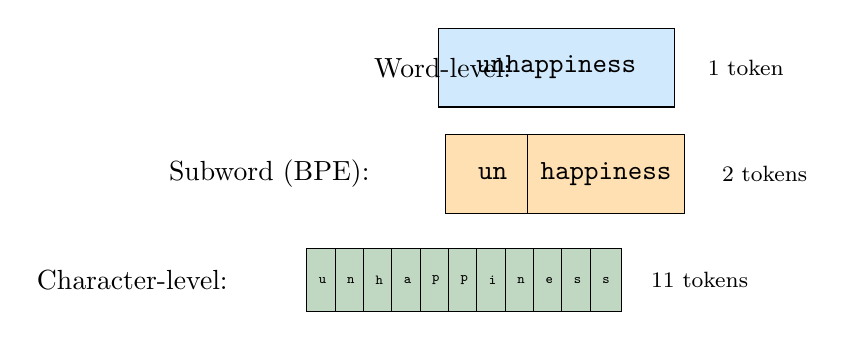
\begin{tikzpicture}[scale=0.9]
            % Word-level
            \node[rectangle, draw, fill=lightblue!30, minimum width=3cm, minimum height=1cm] at (0,3) {\texttt{unhappiness}};
            \node[anchor=east] at (-0.5,3) {Word-level:};
            \node[anchor=west, font=\footnotesize] at (2,3) {1 token};

            % Subword BPE
            \node[rectangle, draw, fill=orange!30, minimum width=1.2cm, minimum height=1cm] at (-0.9,1.5) {\texttt{un}};
            \node[rectangle, draw, fill=orange!30, minimum width=2cm, minimum height=1cm] at (0.7,1.5) {\texttt{happiness}};
            \node[anchor=east] at (-2.5,1.5) {Subword (BPE):};
            \node[anchor=west, font=\footnotesize] at (2.2,1.5) {2 tokens};

            % Character-level
            \node[rectangle, draw, fill=darkgreen!30, minimum width=0.4cm, minimum height=0.8cm] at (-3.3,0) {\tiny \texttt{u}};
            \node[rectangle, draw, fill=darkgreen!30, minimum width=0.4cm, minimum height=0.8cm] at (-2.9,0) {\tiny \texttt{n}};
            \node[rectangle, draw, fill=darkgreen!30, minimum width=0.4cm, minimum height=0.8cm] at (-2.5,0) {\tiny \texttt{h}};
            \node[rectangle, draw, fill=darkgreen!30, minimum width=0.4cm, minimum height=0.8cm] at (-2.1,0) {\tiny \texttt{a}};
            \node[rectangle, draw, fill=darkgreen!30, minimum width=0.4cm, minimum height=0.8cm] at (-1.7,0) {\tiny \texttt{p}};
            \node[rectangle, draw, fill=darkgreen!30, minimum width=0.4cm, minimum height=0.8cm] at (-1.3,0) {\tiny \texttt{p}};
            \node[rectangle, draw, fill=darkgreen!30, minimum width=0.4cm, minimum height=0.8cm] at (-0.9,0) {\tiny \texttt{i}};
            \node[rectangle, draw, fill=darkgreen!30, minimum width=0.4cm, minimum height=0.8cm] at (-0.5,0) {\tiny \texttt{n}};
            \node[rectangle, draw, fill=darkgreen!30, minimum width=0.4cm, minimum height=0.8cm] at (-0.1,0) {\tiny \texttt{e}};
            \node[rectangle, draw, fill=darkgreen!30, minimum width=0.4cm, minimum height=0.8cm] at (0.3,0) {\tiny \texttt{s}};
            \node[rectangle, draw, fill=darkgreen!30, minimum width=0.4cm, minimum height=0.8cm] at (0.7,0) {\tiny \texttt{s}};
            \node[anchor=east] at (-4.5,0) {Character-level:};
            \node[anchor=west, font=\footnotesize] at (1.2,0) {11 tokens};
        \end{tikzpicture}
    \end{center}

    \vspace{0.5em}
    \textbf{Trade-off:} Vocabulary size vs. sequence length
\end{frame}

\begin{frame}[shrink=10]{Byte-Pair Encoding (BPE) 🔧}
    \textbf{Key idea:} Start with characters, iteratively merge frequent pairs

    \vspace{0.5em}
    \textbf{Algorithm:}
    \begin{enumerate}\setlength{\itemsep}{0pt}
        \item Start with vocabulary of all characters
        \item Find most frequent pair of tokens
        \item Merge this pair into a new token
        \item Repeat until desired vocabulary size
    \end{enumerate}

    \vspace{0.5em}
    \textbf{Example progression:}
    \begin{itemize}\setlength{\itemsep}{0pt}
        \item Initial: \texttt{[l, o, w, e, r, ...]}
        \item After merge 1: \texttt{[lo, w, e, r, ...]} (if "lo" is frequent)
        \item After merge 2: \texttt{[low, e, r, ...]} (if "low" is frequent)
        \item After many merges: \texttt{[lower, lowest, ...]}
    \end{itemize}

    \vspace{0.5em}
    📖 \textbf{Reference:} Sennrich et al. (2016) - Neural Machine Translation of Rare Words with Subword Units
\end{frame}

\begin{frame}{Tokenization Methods Comparison 📋}
    \begin{table}
        \centering
        \small
        \begin{tabular}{llll}
            \toprule
            \textbf{Method} & \textbf{Approach} & \textbf{Used By} & \textbf{Key Feature} \\
            \midrule
            BPE & Frequency-based & GPT-2, GPT-3 & Simple, effective \\
            & merging & RoBERTa & \\
            \midrule
            WordPiece & Similar to BPE, & BERT & Likelihood-based \\
            & likelihood scoring & DistilBERT & merging \\
            \midrule
            SentencePiece & Language-agnostic & T5, ALBERT & Works on raw text \\
            & unigram LM & mT5 & (no pre-tokenization) \\
            \bottomrule
        \end{tabular}
    \end{table}

    \vspace{1em}
    📖 \textbf{References:}
    \begin{itemize}\setlength{\itemsep}{0pt}
        \item Kudo \& Richardson (2018) - SentencePiece
        \item \href{https://huggingface.co/learn/nlp-course/chapter2/4}{HuggingFace Chapter 2.4: Tokenizers}
        \item \href{https://huggingface.co/learn/nlp-course/chapter6}{HuggingFace Chapter 6: Tokenizers}
    \end{itemize}
\end{frame}

\begin{frame}[fragile]{Try It: Comparing Tokenizers 💡}
    \begin{lstlisting}[language=Python]
from transformers import AutoTokenizer

text = "I'm learning about tokenization!"

# GPT-2 (BPE)
gpt2_tokenizer = AutoTokenizer.from_pretrained("gpt2")
print("GPT-2:", gpt2_tokenizer.tokenize(text))

# BERT (WordPiece)
bert_tokenizer = AutoTokenizer.from_pretrained("bert-base-uncased")
print("BERT:", bert_tokenizer.tokenize(text))

# T5 (SentencePiece)
t5_tokenizer = AutoTokenizer.from_pretrained("t5-small")
print("T5:", t5_tokenizer.tokenize(text))
    \end{lstlisting}

    \vspace{0.5em}
    \textbf{Your turn!} Try this with different texts and observe:
    \begin{itemize}\setlength{\itemsep}{0pt}
        \item How do they handle punctuation?
        \item What about rare words or typos?
        \item Which produces the shortest sequence?
    \end{itemize}
\end{frame}

% Part-of-Speech Tagging
\begin{frame}[shrink=10]{Part-of-Speech (POS) Tagging 🎯}
    \textbf{What is POS tagging?}
    \begin{itemize}\setlength{\itemsep}{0pt}
        \item Identifying grammatical role of each word
        \item Examples: noun, verb, adjective, adverb, etc.
        \item Crucial for understanding sentence structure
    \end{itemize}

    \vspace{0.5em}
    \textbf{Example:}
    \begin{center}
        \begin{tabular}{lllllll}
            \textbf{Word:} & The & cat & sat & on & the & mat \\
            \textbf{POS:} & DET & NOUN & VERB & ADP & DET & NOUN \\
        \end{tabular}
    \end{center}

    \vspace{0.5em}
    \textbf{Why it matters:}
    \begin{itemize}\setlength{\itemsep}{0pt}
        \item Disambiguation: "book" as noun vs. verb ("Book a table")
        \item Syntax analysis and parsing
        \item Information extraction
        \item Machine translation
    \end{itemize}
\end{frame}

\begin{frame}[fragile]{POS Tagging in Action 🚀}
    \begin{lstlisting}[language=Python]
import spacy

nlp = spacy.load("en_core_web_sm")
doc = nlp("She will book the meeting room tomorrow")

for token in doc:
    print(f"{token.text:10} {token.pos_:6} {spacy.explain(token.pos_)}")

# Output:
# She        PRON   pronoun
# will       AUX    auxiliary
# book       VERB   verb
# the        DET    determiner
# meeting    NOUN   noun
# room       NOUN   noun
# tomorrow   NOUN   noun
    \end{lstlisting}

    \vspace{0.5em}
    Notice "book" is correctly identified as a VERB, not NOUN!
\end{frame}

\begin{frame}[shrink=10]{Syntactic Dependencies in Neural Networks 🧠}
    \textbf{Can neural networks learn grammar?}

    \vspace{0.5em}
    Example from Linzen et al. (2016):
    \begin{itemize}\setlength{\itemsep}{0pt}
        \item "The key to the cabinets \underline{is} on the table" ✓
        \item "The key to the cabinets \underline{are} on the table" ✗
    \end{itemize}

    \vspace{0.5em}
    \textbf{Challenge:} Subject-verb agreement with distractors
    \begin{itemize}\setlength{\itemsep}{0pt}
        \item Model must track "key" (singular) not "cabinets" (plural)
        \item Tests long-range syntactic dependencies
    \end{itemize}

    \vspace{0.5em}
    \textbf{BLiMP Dataset} (Warstadt et al. 2020):
    \begin{itemize}\setlength{\itemsep}{0pt}
        \item Benchmark of Linguistic Minimal Pairs
        \item 67 tasks covering syntax, semantics, morphology
        \item Tests if models have implicit grammatical knowledge
    \end{itemize}

    \vspace{0.5em}
    📖 \textbf{Resources:} \href{https://huggingface.co/learn/nlp-course/chapter7/2}{HuggingFace Chapter 7.2: Token Classification}
\end{frame}

\begin{frame}{Discussion: Grammar Without Rules? 🤔}
    \textbf{Traditional linguistics:} Explicit grammatical rules (Chomsky)

    \textbf{Neural networks:} Implicit patterns from data

    \vspace{1em}
    \textbf{Questions to ponder:}
    \begin{enumerate}\setlength{\itemsep}{0pt}
        \item Do neural networks "learn" grammar the same way humans do?
        \item Can statistical patterns capture syntactic knowledge?
        \item What does it mean to "understand" grammar?
        \item Are there linguistic phenomena that pure statistics can't capture?
    \end{enumerate}

    \vspace{1em}
    \textbf{Cognitive connection:} Children learn grammar without explicit rules—just exposure to language. How similar are they to neural networks?
\end{frame}

% Sentiment Analysis
\begin{frame}[shrink=10]{Sentiment Analysis 😊😢}
    \textbf{What is sentiment analysis?}
    \begin{itemize}\setlength{\itemsep}{0pt}
        \item Determining emotional tone of text
        \item Classification task: positive, negative, neutral
        \item Can be fine-grained (1-5 stars) or coarse (binary)
    \end{itemize}

    \vspace{0.5em}
    \textbf{Applications:}
    \begin{itemize}\setlength{\itemsep}{0pt}
        \item Customer feedback analysis
        \item Social media monitoring
        \item Market research
        \item Political opinion tracking
    \end{itemize}

    \vspace{0.5em}
    \textbf{Challenges:}
    \begin{itemize}\setlength{\itemsep}{0pt}
        \item Sarcasm: "Oh great, another meeting 🙄"
        \item Context-dependence: "This movie is sick!" (positive in slang)
        \item Mixed sentiments: "The food was great but service was terrible"
    \end{itemize}
\end{frame}

\begin{frame}[fragile]{Sentiment Analysis with HuggingFace 🤗}
    \begin{lstlisting}[language=Python]
from transformers import pipeline

# Load sentiment analysis pipeline
sentiment_analyzer = pipeline("sentiment-analysis")

# Analyze some texts
texts = [
    "I love this product! It's amazing!",
    "This is the worst experience ever.",
    "It's okay, nothing special."
]

for text in texts:
    result = sentiment_analyzer(text)[0]
    print(f"Text: {text}")
    print(f"Sentiment: {result['label']}, Score: {result['score']:.3f}\n")

# Output:
# Text: I love this product! It's amazing!
# Sentiment: POSITIVE, Score: 0.999
#
# Text: This is the worst experience ever.
# Sentiment: NEGATIVE, Score: 0.998
    \end{lstlisting}
\end{frame}

\begin{frame}[shrink=10]{Fine-tuning for Sentiment Analysis 🎯}
    \textbf{Pre-trained models} are trained on general text

    \textbf{Fine-tuning} adapts them to specific domains:
    \begin{itemize}\setlength{\itemsep}{0pt}
        \item Movie reviews (IMDb dataset)
        \item Product reviews (Amazon)
        \item Financial news sentiment
        \item Medical patient feedback
    \end{itemize}

    \vspace{0.5em}
    \textbf{Process:}
    \begin{enumerate}\setlength{\itemsep}{0pt}
        \item Start with pre-trained model (e.g., BERT)
        \item Add classification layer
        \item Train on labeled sentiment data
        \item Evaluate on test set
    \end{enumerate}

    \vspace{0.5em}
    📖 \textbf{Resources:}
    \begin{itemize}\setlength{\itemsep}{0pt}
        \item \href{https://huggingface.co/learn/nlp-course/chapter1/2}{HuggingFace Chapter 1.2: NLP Tasks}
        \item \href{https://huggingface.co/learn/nlp-course/chapter3/2}{HuggingFace Chapter 3.2: Processing Data}
    \end{itemize}
\end{frame}

\begin{frame}[fragile]{Try It: Domain-Specific Sentiment 💡}
    \begin{lstlisting}[language=Python]
from transformers import pipeline

# General sentiment
general_analyzer = pipeline("sentiment-analysis")

# Financial sentiment (specialized model)
finbert = pipeline("sentiment-analysis",
                   model="ProsusAI/finbert")

text = "The company's earnings exceeded expectations"

print("General:", general_analyzer(text))
print("Financial:", finbert(text))
    \end{lstlisting}

    \vspace{0.5em}
    \textbf{Your challenge:} Find domain-specific sentiment models on HuggingFace Hub:
    \begin{itemize}\setlength{\itemsep}{0pt}
        \item Twitter sentiment
        \item Product reviews
        \item Movie reviews
    \end{itemize}
    Compare their predictions on the same text!
\end{frame}

% Statistical Learning in Infants
\begin{frame}[shrink=10]{Statistical Learning in Infants 👶}
    \textbf{How do babies learn language?}

    \vspace{0.5em}
    \textbf{Classic study:} Saffran et al. (1996)
    \begin{itemize}\setlength{\itemsep}{0pt}
        \item 8-month-old infants exposed to artificial language
        \item Continuous stream: \textit{bidakupadotigolabubidaku...}
        \item No pauses between "words"
        \item Only cue: statistical regularities (transitional probabilities)
    \end{itemize}

    \vspace{0.5em}
    \textbf{Key findings:}
    \begin{itemize}\setlength{\itemsep}{0pt}
        \item Infants could segment words from continuous speech
        \item They tracked which syllables frequently occur together
        \item \textit{bidaku} (high transitional probability) → word
        \item \textit{kupado} (low transitional probability) → word boundary
    \end{itemize}

    \vspace{0.5em}
    \textbf{Implication:} Statistical learning is a fundamental mechanism for language acquisition!
\end{frame}

\begin{frame}[shrink=5]{Statistical Regularities: The Numbers 📊}
    \textbf{Transitional Probability:} $P(\text{syllable}_2 | \text{syllable}_1)$

    \vspace{0.5em}
    \textbf{Example from Saffran et al. (1996):}

    \begin{center}
        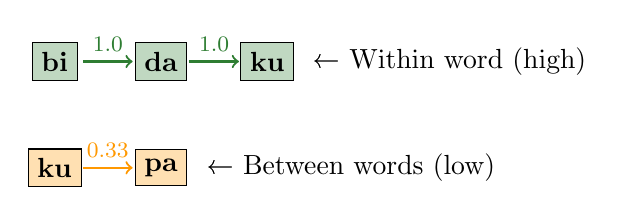
\begin{tikzpicture}[scale=0.9]
            % Within-word transitions (high probability)
            \node[rectangle, draw, fill=darkgreen!30] at (0,2) {\textbf{bi}};
            \node[rectangle, draw, fill=darkgreen!30] at (1.5,2) {\textbf{da}};
            \node[rectangle, draw, fill=darkgreen!30] at (3,2) {\textbf{ku}};
            \draw[->, thick, color=darkgreen] (0.4,2) -- (1.1,2) node[midway,above,font=\footnotesize] {1.0};
            \draw[->, thick, color=darkgreen] (1.9,2) -- (2.6,2) node[midway,above,font=\footnotesize] {1.0};
            \node[anchor=west] at (3.5,2) {← Within word (high)};

            % Between-word transitions (low probability)
            \node[rectangle, draw, fill=orange!30] at (0,0.5) {\textbf{ku}};
            \node[rectangle, draw, fill=orange!30] at (1.5,0.5) {\textbf{pa}};
            \draw[->, thick, color=orange] (0.4,0.5) -- (1.1,0.5) node[midway,above,font=\footnotesize] {0.33};
            \node[anchor=west] at (2,0.5) {← Between words (low)};
        \end{tikzpicture}
    \end{center}

    \vspace{0.5em}
    Infants learned to recognize:
    \begin{itemize}\setlength{\itemsep}{0pt}
        \item High probability → within-word transitions
        \item Low probability → word boundaries
    \end{itemize}

    \vspace{0.5em}
    📖 \textbf{Reference:} Saffran, Aslin, \& Newport (1996) - Statistical learning by 8-month-old infants
\end{frame}

\begin{frame}[shrink=10]{Connecting Infants to NLP 🔄}
    \begin{columns}[T]
        \begin{column}{0.48\textwidth}
            \textbf{👶 Infant Learning:}
            \begin{itemize}\setlength{\itemsep}{0pt}
                \item Track syllable co-occurrence
                \item Learn word boundaries
                \item No explicit supervision
                \item Pattern recognition
                \item Limited exposure (hours)
            \end{itemize}
        \end{column}
        \begin{column}{0.48\textwidth}
            \textbf{🤖 Neural Networks:}
            \begin{itemize}\setlength{\itemsep}{0pt}
                \item Track token co-occurrence
                \item Learn subword units (BPE)
                \item Self-supervised learning
                \item Statistical patterns
                \item Massive exposure (billions of words)
            \end{itemize}
        \end{column}
    \end{columns}

    \vspace{1em}
    \textbf{Discussion Questions:}
    \begin{enumerate}\setlength{\itemsep}{0pt}
        \item Are these processes fundamentally similar?
        \item What do infants have that models don't? (social cues, multimodal input...)
        \item What do models have that infants don't? (scale, perfect memory...)
        \item Can statistical learning alone explain language acquisition?
    \end{enumerate}
\end{frame}

\begin{frame}{From Statistical Learning to Modern Tokenization 🔍}
    \textbf{Parallel ideas:}

    \begin{center}
        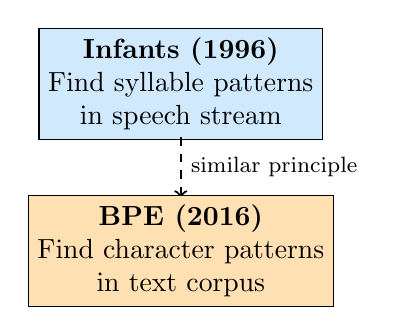
\begin{tikzpicture}[scale=0.85]
            % Infants
            \node[rectangle, draw, fill=lightblue!30, minimum width=3.5cm, minimum height=1.2cm, align=center] at (0,3)
                {\textbf{Infants (1996)} \\ Find syllable patterns \\ in speech stream};

            % Arrow
            \draw[->, thick, dashed] (0,2.2) -- (0,1.3) node[midway,right,font=\footnotesize] {similar principle};

            % BPE
            \node[rectangle, draw, fill=orange!30, minimum width=3.5cm, minimum height=1.2cm, align=center] at (0,0.5)
                {\textbf{BPE (2016)} \\ Find character patterns \\ in text corpus};
        \end{tikzpicture}
    \end{center}

    \vspace{0.5em}
    \textbf{Key similarity:} Both use \textit{distributional statistics} to discover structure

    \vspace{0.5em}
    \textbf{Key difference:}
    \begin{itemize}\setlength{\itemsep}{0pt}
        \item Infants: Real-time, online learning with multimodal cues
        \item BPE: Batch processing of text, no other modalities
    \end{itemize}
\end{frame}

% Practical Exercises
\begin{frame}[shrink=10]{Hands-On Practice 🛠️}
    \textbf{Today's demos covered:}
    \begin{enumerate}\setlength{\itemsep}{0pt}
        \item \textbf{Web scraping} with Beautiful Soup
        \item \textbf{Lemmatization} with spaCy
        \item \textbf{Tokenization} comparison (GPT-2, BERT, T5)
        \item \textbf{POS tagging} with spaCy
        \item \textbf{Sentiment analysis} with HuggingFace
    \end{enumerate}

    \vspace{1em}
    \textbf{Try combining them!} 💡
    \begin{itemize}\setlength{\itemsep}{0pt}
        \item Scrape news articles → analyze sentiment trends
        \item Lemmatize text → compare tokenization results
        \item POS tag → extract only nouns and verbs → analyze
    \end{itemize}
\end{frame}

\begin{frame}[fragile]{Mini-Project Idea: News Sentiment Tracker 📰}
    \begin{lstlisting}[language=Python]
# Combine all techniques!
from bs4 import BeautifulSoup
import requests
from transformers import pipeline

# 1. Scrape news
url = "https://news.ycombinator.com"
response = requests.get(url)
soup = BeautifulSoup(response.content, 'html.parser')
headlines = [title.get_text() for title in soup.find_all('span', class_='titleline')]

# 2. Analyze sentiment
sentiment_analyzer = pipeline("sentiment-analysis")

# 3. Aggregate results
positive_count = 0
for headline in headlines[:10]:
    result = sentiment_analyzer(headline)[0]
    if result['label'] == 'POSITIVE':
        positive_count += 1
    print(f"{headline[:50]}: {result['label']}")

print(f"\n{positive_count}/10 headlines are positive")
    \end{lstlisting}
\end{frame}

% Assignment 2
\begin{frame}[shrink=10]{Assignment 2: SPAM Email Classifier 📧}
    \textbf{Your task:} Build a classifier to detect spam emails

    \vspace{0.5em}
    \textbf{What you'll practice:}
    \begin{itemize}\setlength{\itemsep}{0pt}
        \item Data cleaning and preprocessing
        \item Text tokenization
        \item Feature extraction
        \item Training a classification model
        \item Evaluating performance
    \end{itemize}

    \vspace{0.5em}
    \textbf{Skills you'll use:}
    \begin{itemize}\setlength{\itemsep}{0pt}
        \item Everything from today's lecture!
        \item Lemmatization to normalize words
        \item Tokenization to handle different vocabularies
        \item Sentiment-like classification (spam vs. ham)
    \end{itemize}

    \vspace{0.5em}
    \textbf{Link:} \href{https://github.com/ContextLab/llm-course/tree/main/assignments/Assignment\%202\%3A\%20SPAM\%20classifier}{Assignment 2: SPAM classifier}
\end{frame}

\begin{frame}[shrink=10]{Assignment 2: Getting Started 🚀}
    \textbf{Suggested approach:}
    \begin{enumerate}\setlength{\itemsep}{0pt}
        \item \textbf{Explore the data:} What do spam vs. legitimate emails look like?
        \item \textbf{Preprocess:} Clean HTML, remove special characters, lemmatize
        \item \textbf{Tokenize:} Try different tokenization strategies
        \item \textbf{Extract features:} Bag of words? TF-IDF? Word embeddings?
        \item \textbf{Train classifier:} Start simple (Naive Bayes), then try others
        \item \textbf{Evaluate:} Accuracy, precision, recall, F1-score
        \item \textbf{Iterate:} Improve based on error analysis
    \end{enumerate}

    \vspace{0.5em}
    \textbf{Think about:}
    \begin{itemize}\setlength{\itemsep}{0pt}
        \item What features distinguish spam from legitimate emails?
        \item How does preprocessing affect performance?
        \item What mistakes does your classifier make?
    \end{itemize}
\end{frame}

% Conclusion and Discussion
\begin{frame}[shrink=10]{Key Takeaways 🎯}
    \begin{enumerate}\setlength{\itemsep}{0pt}
        \item \textbf{Preprocessing matters:} Clean data = better results
        \item \textbf{Tokenization is fundamental:} Choice affects everything downstream
        \item \textbf{Subword tokenization:} Balances vocabulary size and semantic coverage
        \item \textbf{Statistical learning:} Core principle in both humans and machines
        \item \textbf{Multiple levels of analysis:} Characters → subwords → words → syntax → semantics
    \end{enumerate}

    \vspace{1em}
    \textbf{The Big Picture:}
    \begin{itemize}\setlength{\itemsep}{0pt}
        \item Computational methods can model linguistic phenomena
        \item But: Are they modeling the \textit{same} processes as humans?
        \item Statistical patterns are powerful, but is there more to language?
    \end{itemize}
\end{frame}

\begin{frame}[shrink=10]{Looking Ahead: Week 3-4 🔮}
    \textbf{Next topics:}
    \begin{itemize}\setlength{\itemsep}{0pt}
        \item Dimensionality reduction (PCA, UMAP)
        \item Bag-of-words models
        \item Word embeddings (Word2Vec, GloVe)
        \item Distributional semantics: "You shall know a word by the company it keeps"
    \end{itemize}

    \vspace{1em}
    \textbf{Prepare by:}
    \begin{itemize}\setlength{\itemsep}{0pt}
        \item Completing Assignment 2
        \item Reading about distributional semantics
        \item Thinking about: How can we represent word \textit{meaning}?
    \end{itemize}
\end{frame}

\begin{frame}[shrink=10]{Additional Resources 📚}
    \textbf{Primary Sources:}
    \begin{itemize}\setlength{\itemsep}{0pt}
        \item Sennrich et al. (2016) - BPE for neural machine translation
        \item Kudo \& Richardson (2018) - SentencePiece
        \item Linzen et al. (2016) - LSTMs and syntax
        \item Warstadt et al. (2020) - BLiMP benchmark
        \item Saffran et al. (1996) - Statistical learning in infants
    \end{itemize}

    \vspace{0.5em}
    \textbf{HuggingFace Resources:}
    \begin{itemize}\setlength{\itemsep}{0pt}
        \item Chapter 2.4: Behind the Pipeline - Tokenizers
        \item Chapter 6: Tokenizers (full chapter)
        \item Chapter 7.2: Token Classification
        \item Chapter 1.2: NLP Tasks with Pipeline
        \item Chapter 3.2: Processing Data for Fine-tuning
    \end{itemize}
\end{frame}

\begin{frame}{Discussion: Open Questions 💭}
    \textbf{To think about:}

    \begin{enumerate}\setlength{\itemsep}{0pt}
        \item If a model can perform POS tagging without explicit grammatical rules, does it "understand" grammar?

        \item Infants learn from \textasciitilde 10M words by age 3. Models train on billions. What does this tell us?

        \item Can statistical co-occurrence alone explain semantic understanding?

        \item What aspects of language might require more than pattern matching?

        \item How should we interpret model "knowledge" vs. human knowledge?
    \end{enumerate}

    \vspace{1em}
    \textbf{Keep these questions in mind as we progress through the course!}
\end{frame}

\begin{frame}[standout]
    \Huge Thank you! 🎉

    \vspace{1em}

    \large Questions?

    \vspace{1em}

    \normalsize
    Next week: Dimensionality Reduction \& Word Embeddings
\end{frame}

\end{document}
